%%%%%%%%%%%%%%%%%%%%%%%%%%%%%%%%% Search Space %%%%%%%%%%%%%%%%%%
\begin{frame}{Espace de Recherche}

    \begin{table}[h]
        \centering
        \begin{tabular}{|c|c|c|c|c|}
            \hline
            \multirow{2}{*}{\textbf{ Hyperparamètres }} & \multicolumn{2}{|c|}{\textbf{Plage d'Optimisation}} &\multirow{2}{*}{\textbf{ Type }}& \multirow{2}{*}{\textbf{ Conversion }} \\
            \cline{2-3}
             & \textbf{ Borne Inf. } & \textbf{ Borne Sup. } & & \\
            \hline
            \textbf{Learning Rate} & $-10$ & $-1$ & log. & $f(x) = 10^{x}$ \\
            \hline
            \textbf{LoRA rank} & 1 & 64 &ent. &$f(x) = \text{round}(x)$ \\
            \hline
            \textbf{LoRA scale} &1 & 64 & ent. &$f(x) = \text{round}(x)$ \\
            \hline
            \textbf{Dropout} & 0 & 0.5 & cont.& $f(x) = x$ \\
            \hline
            \textbf{Weight Decay} & $-3$ & $-1$ &log.& $f(x) = 10^{x}$  \\
            \hline
        \end{tabular}
        \caption{Résumé de l'espace de recherche}
    \end{table}

    \begin{itemize}
        \item Variables mixes : étape de conversion nécessaire
    \end{itemize}

\end{frame}

%%%%%%%%%%%%%%%%%%%%%%%%%%%%%%%%% Search Strategy : BO %%%%%%%%%%%%%%%%%%
\begin{frame}{Strategie de Recherche : Optimisation Bayésienne par Process Gaussien }
    \begin{columns}
    %%%%%%%%%%%%%%%%%%%%%%%%%% COLONNE DE GAUCHE %%%%%%%%%%%%%%
    \begin{column}[t]{0.4\textwidth} 
        \begin{block}{Algorithm}
                \begin{itemize}
                    \item Echantillon de $n$ Points (LHS)
                    \item Evaluer ces $n$ points
                    \item Jusqu'à fin du budget
                    \begin{itemize}
                        \item Entrainer le Process Gaussien (GP)
                        \item Optimiser ce GP pour obtenir un nouveau Point
                        \item Evaluer ce nouveaux point
                    \end{itemize}
                \end{itemize}
        \end{block}
 
        \end{column}
             
     %%%%%%%%%%%%%%%%%%%%%%%%% COLONNE DE DROITE %%%%%%%%%%%%%%
        \begin{column}[t]{0.6\textwidth}
            \begin{figure}
                \centering
                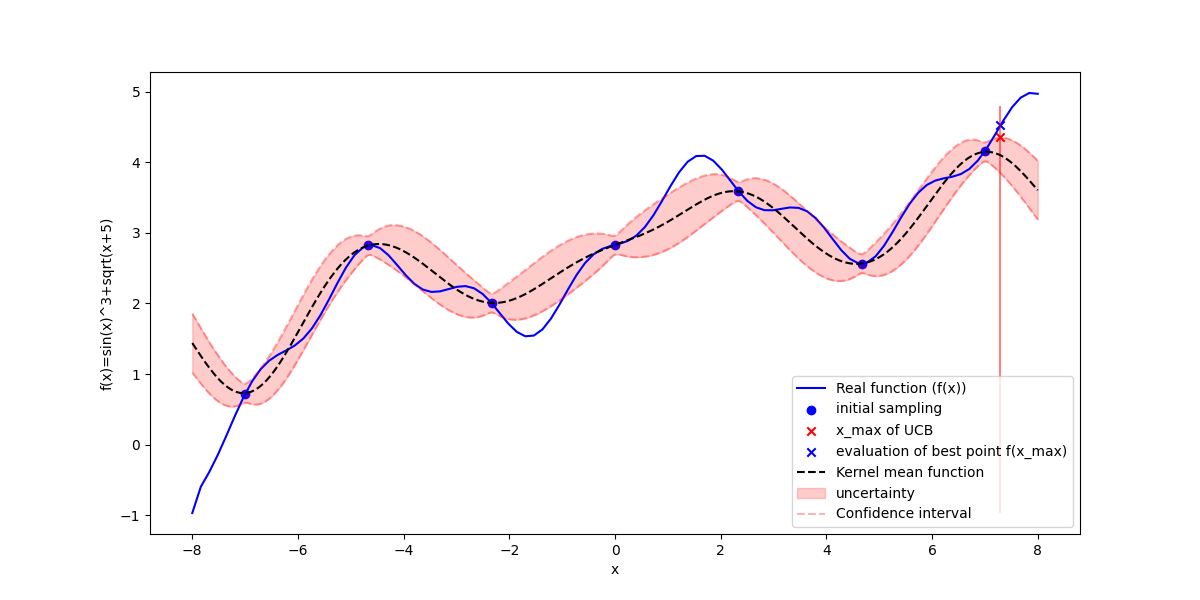
\includegraphics[width = \textwidth]{assets/imgs/gaussian_process.png}
                \caption{Example d'un surrogate sur une fonction en 1D}
            \end{figure} 
        \end{column}
             
    \end{columns}

\end{frame}

%%%%%%%%%%%%%%%%%%%%%%%%%%%%%%%%% Search Strategy : SOO %%%%%%%%%%%%%%%%%%
\begin{frame}{Strategie de Recherche : Simultaneous Optimistic Optimization (SOO)}
    \begin{columns}
        %%%%%%%%%%%%%%%%%%%%%%%%%% COLONNE DE GAUCHE %%%%%%%%%%%%%%
        \begin{column}[t]{0.5\textwidth} 
            \begin{figure}
                \centering
                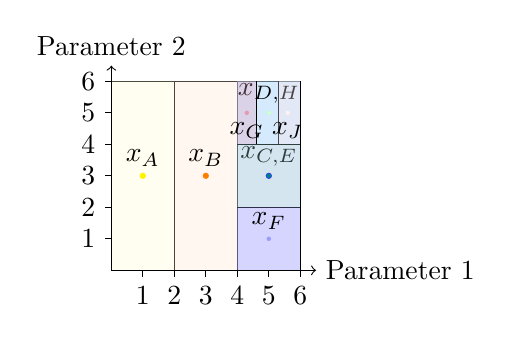
\begin{tikzpicture}[scale=0.4]

    % Define the grid
    \draw[step=6,black,very thin] (0,0) grid (6,6);

    
    % first decomposition
    \draw (2,0) -- (2,6) ;
    \draw (4,0) -- (4,6);
        % point A
        \fill[yellow!20, opacity = 0.3] (0.0,0) rectangle (2,6);
        \fill[fill = yellow] (1,3) circle (0.1) node[above]{$x_A$};  % Point in the first square
        
        % point B
        \fill[orange!20, opacity = 0.3] (2,0) rectangle (4,6);
        \fill[fill = orange] (3,3) circle (0.1) node[above]{$x_B$};  % Point in the first square
        % point C
        \fill[blue!20, opacity = 0.3] (4,0) rectangle (6,6);
        \fill[fill = blue] (5,3) circle (0.1) node[above]{$x_{C,E}$};  % Point in the first square

    % second decomposition
    \draw (4,2) -- (6,2);
    \draw (4,4) -- (6,4);
      % point D
      \fill[cyan!40, opacity = 0.3] (4,4) rectangle (6,6);
      \fill[fill = cyan!40] (5,5) circle (0.07) node[above]{$x_{D,H}$} ;  % Point in the first square
      %point E
      \fill[teal!40, opacity = 0.3] (4,2) rectangle (6,4);
      \fill[fill = teal] (5,3) circle (0.07) ;  % Point in the first square
      %point F
      \fill[blue!40, opacity = 0.3] (4,0) rectangle (6,2);
      \fill[fill = blue!40] (5,1) circle (0.07) node[above]{$x_F$} ;  % Point in the first square

    % second decomposition
    \draw (4.6,4) -- (4.6,6);
    \draw (5.3,4) -- (5.3,6);
      %point G
      \fill[purple!40, opacity = 0.3] (4,4) rectangle (4.6,6);
      \fill[fill = purple!40] (4.3,5) circle (0.07) node[below]{$x_G$} ;  % Point in the first square
      %point H
      %\fill[green!40, opacity = 0.3] (4.6,4) rectangle (5.3,6);
      \fill[fill = green!20] (5,5) circle (0.07);  % Point in the first square
      %point J
      \fill[pink!40, opacity = 0.3] (5.3,4) rectangle (6,6);
      \fill[fill = pink!20] (5.6,5) circle (0.07) node[below]{$x_J$} ;  % Point in the first square
    

    % Draw red points
    \fill[red] (3,3) circle (0.01);  % Point in the first square

    
    % Draw the axes
    \draw[->] (0,0) -- (6.5,0) node[right] {Parameter 1};
    \draw[->] (0,0) -- (0,6.5) node[above] {Parameter 2};
    
    % Add ticks and labels
    \foreach \x in {1,2,3,4,5,6} {
      \draw (\x,0) -- (\x,-0.2) node[below] {\x};
      \draw (0,\x) -- (-0.2,\x) node[left] {\x};
    }
    
\end{tikzpicture}
                \caption{Partition de l'espace de recherche par SOO}
            \end{figure} 
     
            \end{column}
                 
         %%%%%%%%%%%%%%%%%%%%%%%%% COLONNE DE DROITE %%%%%%%%%%%%%%
            \begin{column}[t]{0.5\textwidth}
                \begin{figure}
                    \centering
                    \begin{tikzpicture}[]
    \tikzstyle{space} = [circle, minimum width=0.6cm,text centered, draw=black]
    \tikzstyle{arrow} = [thick,->,>=stealth]

      \node(space)[space, fill = purple!50]{$\Omega$};


 
        %depth 1
        \node(B)[space, fill = magenta!40, below of = space, yshift = -0cm]{B};
        \node(A)[space, fill = red!50, left of = B, xshift = -10pt]{A};
        \node(C)[space, fill = teal!50,  right of = B, xshift = 10pt]{C};
        \draw[arrow] (space) -- (A);
        \draw[arrow] (space) -- (B);
        \draw[arrow] (space) -- (C);

    \onslide<1>{
      \node (fit_A,B,C)[draw, thick, dashed, rounded corners, fit=(A)(B)(C), inner sep=0.1cm] {};
    }
    
    \onslide<2->{ % First loop
    %depth 1
    \node(E)[space, fill = teal!40, below of = C, yshift = -0cm]{E};
    \node(D)[space, fill = blue!50, left of = E]{D};
    \node(F)[space, fill = olive!40,  right of = E]{F};
    \draw[arrow] (C) -- (E);
    \draw[arrow] (C) -- (D);
    \draw[arrow] (C) -- (F);

    }
    \onslide<2>{
      \node (fit_E_D_F)[draw, thick, dashed, rounded corners, fit=(E)(D)(F), inner sep=0.1cm] {};
    }

    \onslide<3->{
    %depth 2
    \node(H)[space, fill = red!20, below of = A]{H};
    \node(G)[space, fill = orange!50, left of = H]{G};
    \node(I)[space, fill = pink!80,  right of = H]{I};
    \draw[arrow] (A) -- (G);
    \draw[arrow] (A) -- (H);
    \draw[arrow] (A) -- (I);

    \node(K)[space, fill = cyan!50, below of = D]{K};
    \node(J)[space, fill = blue!20, left of = K]{J};
    \node(L)[space, fill = cyan!20,  right of = K]{L};
    \draw[arrow] (D) -- (J);
    \draw[arrow] (D) -- (K);
    \draw[arrow] (D) -- (L);

    \node (fit_G_H_I)[draw, thick, dashed, rounded corners, fit=(G)(H)(I), inner sep=0.1cm] {};
    \node (fit_J_K_L)[draw, thick, dashed, rounded corners, fit=(J)(K)(L), inner sep=0.1cm] {};

    }
    
    

\end{tikzpicture}
                    \caption{Arbre correspondant à SOO}
                \end{figure} 
            \end{column}
                 
    \end{columns}

\end{frame}

%%%%%%%%%%%%%%%%%%%%%%%%%%%%%%%%% Search Strategy : BaMSOO %%%%%%%%%%%%%%%%%%
\begin{frame}{Search Strategy : BaMSOO (TO DO)}
    \begin{columns}
        %%%%%%%%%%%%%%%%%%%%%%%%%% COLONNE DE GAUCHE %%%%%%%%%%%%%%
        \begin{column}[t]{0.5\textwidth} 
            \begin{figure}
                \centering
                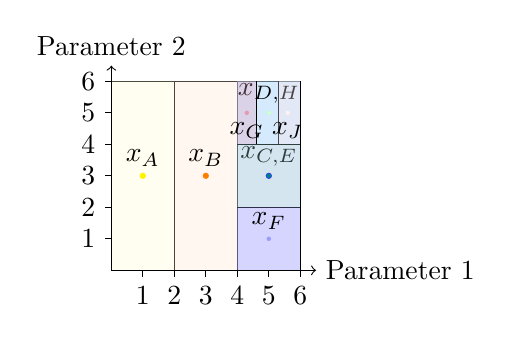
\begin{tikzpicture}[scale=0.4]

    % Define the grid
    \draw[step=6,black,very thin] (0,0) grid (6,6);

    
    % first decomposition
    \draw (2,0) -- (2,6) ;
    \draw (4,0) -- (4,6);
        % point A
        \fill[yellow!20, opacity = 0.3] (0.0,0) rectangle (2,6);
        \fill[fill = yellow] (1,3) circle (0.1) node[above]{$x_A$};  % Point in the first square
        
        % point B
        \fill[orange!20, opacity = 0.3] (2,0) rectangle (4,6);
        \fill[fill = orange] (3,3) circle (0.1) node[above]{$x_B$};  % Point in the first square
        % point C
        \fill[blue!20, opacity = 0.3] (4,0) rectangle (6,6);
        \fill[fill = blue] (5,3) circle (0.1) node[above]{$x_{C,E}$};  % Point in the first square

    % second decomposition
    \draw (4,2) -- (6,2);
    \draw (4,4) -- (6,4);
      % point D
      \fill[cyan!40, opacity = 0.3] (4,4) rectangle (6,6);
      \fill[fill = cyan!40] (5,5) circle (0.07) node[above]{$x_{D,H}$} ;  % Point in the first square
      %point E
      \fill[teal!40, opacity = 0.3] (4,2) rectangle (6,4);
      \fill[fill = teal] (5,3) circle (0.07) ;  % Point in the first square
      %point F
      \fill[blue!40, opacity = 0.3] (4,0) rectangle (6,2);
      \fill[fill = blue!40] (5,1) circle (0.07) node[above]{$x_F$} ;  % Point in the first square

    % second decomposition
    \draw (4.6,4) -- (4.6,6);
    \draw (5.3,4) -- (5.3,6);
      %point G
      \fill[purple!40, opacity = 0.3] (4,4) rectangle (4.6,6);
      \fill[fill = purple!40] (4.3,5) circle (0.07) node[below]{$x_G$} ;  % Point in the first square
      %point H
      %\fill[green!40, opacity = 0.3] (4.6,4) rectangle (5.3,6);
      \fill[fill = green!20] (5,5) circle (0.07);  % Point in the first square
      %point J
      \fill[pink!40, opacity = 0.3] (5.3,4) rectangle (6,6);
      \fill[fill = pink!20] (5.6,5) circle (0.07) node[below]{$x_J$} ;  % Point in the first square
    

    % Draw red points
    \fill[red] (3,3) circle (0.01);  % Point in the first square

    
    % Draw the axes
    \draw[->] (0,0) -- (6.5,0) node[right] {Parameter 1};
    \draw[->] (0,0) -- (0,6.5) node[above] {Parameter 2};
    
    % Add ticks and labels
    \foreach \x in {1,2,3,4,5,6} {
      \draw (\x,0) -- (\x,-0.2) node[below] {\x};
      \draw (0,\x) -- (-0.2,\x) node[left] {\x};
    }
    
\end{tikzpicture}
                \caption{Partition de l'espace de recherche par SOO}
            \end{figure} 
     
            \end{column}
                 
         %%%%%%%%%%%%%%%%%%%%%%%%% COLONNE DE DROITE %%%%%%%%%%%%%%
            \begin{column}[t]{0.5\textwidth}
                \begin{figure}
                    \centering
                    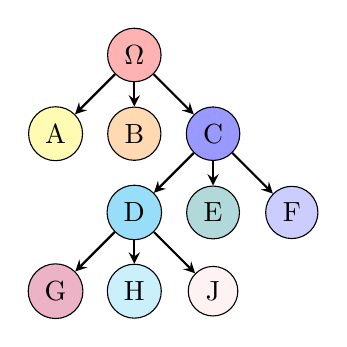
\begin{tikzpicture}[]
    \tikzstyle{space} = [circle, minimum width=1,text centered, draw=black]
    \tikzstyle{arrow} = [thick,->,>=stealth]

    \node(space)[space, fill = red!30]{$\Omega$};

    %depth 1
    \node(B)[space, fill = orange!30, below of = space, yshift = -0cm]{B};
    \node(A)[space, fill = yellow!30, left of = B]{A};
    \node(C)[space, fill = blue!40,  right of = B]{C};
    \draw[arrow] (space) -- (A);
    \draw[arrow] (space) -- (B);
    \draw[arrow] (space) -- (C);

    %depth 1
    \node(E)[space, fill = teal!30, below of = C, yshift = -0cm]{E};
    \node(D)[space, fill = cyan!40, left of = E]{D};
    \node(F)[space, fill = blue!20,  right of = E]{F};
    \draw[arrow] (C) -- (E);
    \draw[arrow] (C) -- (D);
    \draw[arrow] (C) -- (F);

    %depth 2
    \node(H)[space, fill = cyan!20, below of = D]{H};
    \node(G)[space, fill = purple!30, left of = H]{G};
    \node(J)[space, fill = pink!20,  right of = H]{J};
    \draw[arrow] (D) -- (G);
    \draw[arrow] (D) -- (H);
    \draw[arrow] (D) -- (J);


\end{tikzpicture}
                    \caption{Arbre correspondant à SOO}
                \end{figure} 
            \end{column}
                 
    \end{columns}
\end{frame}

%%%%%%%%%%%%%%%%%%%%%%%%%%%%%%%%% Search Strategy : Performance Estimation Strategy %%%%%%%%%%%%%%%%%%
\begin{frame}{Stratégie d'Evaluation de Solutions}
    \begin{block}{Implémentation}
        \begin{itemize}
            \item Fine Tuning
            \begin{itemize}
                \item modèle : LlaMa-3.2-1B
                \item 
            \end{itemize}
            \item Evaluation
            \begin{itemize}
                \item librairie lm\_eval
                \item Evaluation par la précision sur des jeu de données Benchmark : Hellaswag et MMLU
            \end{itemize}
        \end{itemize}

        
    \end{block}

\end{frame}

%%%%%%%%%%%%%%%%%%%%%%%%%%%%%%%%% Implementation %%%%%%%%%%%%%%%%%%
\begin{frame}{Implémentation}
    \begin{columns}
        %%%%%%%%%%%%%%%%%%%%%%%%%% COLONNE DE GAUCHE %%%%%%%%%%%%%%
        \begin{column}[t]{0.45\textwidth} 
            \begin{block}{}
                
                \begin{itemize}
                    \item Programmation Orienté Object en Python
                    \item Travail de documentation : \textit{readme}, indication de type...
                    \item Objectif : permettre le réusage
                    \item Utilisable en ligne de commande pour Grid5000
                \end{itemize}
            \end{block}
     
            \end{column}
                 
         %%%%%%%%%%%%%%%%%%%%%%%%% COLONNE DE DROITE %%%%%%%%%%%%%%
            \begin{column}[t]{0.45\textwidth}
                \begin{figure}
                    \centering
                    \begin{tikzpicture}
    \tikzstyle{class} = [rectangle, draw, text centered, fill = blue!20]
    \tikzstyle{inherit} = [thick,dotted,->,>=stealth]
    \tikzstyle{association} = [thick,->,>=stealth]
    

    % Optimisation package
    \node(algo)[class]{OptAlgo};
    \node(soo)[class, below left of = algo]{SOO};
    \node(bo)[class, below right of = algo]{BO};
    \node(bamsoo)[class, below of = algo, yshift = -1cm]{BaMSOO};

    \draw[inherit] (soo) -- (algo);
    \draw[inherit] (bo) -- (algo);
    \draw[inherit] (bamsoo) -- (soo);
    \draw[inherit] (bamsoo) -- (bo);

    \begin{scope}[on background layer]
        \node(optimization)[draw, thick,fill=black!10,opacity=0.5,on background layer, draw=black!70, dashed, rounded corners, fit=(algo)(bamsoo)(bo)(soo), inner sep=0.15cm, label=above:{Optimisation}] {};
    \end{scope}

    % Search Space
    \node (space)[class, right of = algo, xshift = 2cm]{Search Space};
    \node (solution)[class, below left of = space]{Solution};
    \node (var)[class, below right of = space]{Var};

    \draw[inherit] (solution) -- (space);
    \draw[inherit] (var) -- (space);

    \begin{scope}[on background layer]
        \node(search_space)[draw, thick,fill=black!10,opacity=0.5,on background layer, draw=black!70, dashed, rounded corners, fit=(space)(solution)(var), inner sep=0.15cm, label=above:{Search Space}] {};
    \end{scope}

    % Evaluation
    \node (evaluation)[class, below of = space, yshift = -0.8cm]{Evaluation};

    \begin{scope}[on background layer]
        \node(search_space)[draw, thick,fill=black!10,opacity=0.5,on background layer, draw=black!70, dashed, rounded corners, fit=(evaluation), inner sep=0.15cm, label=below:{Evaluation}] {};
    \end{scope}

    % Association arrow
    \draw[association] (evaluation.west) -- ([xshift=-0.85cm]evaluation.west) -- ([xshift=-0.85cm, yshift = 1.8cm]evaluation.west) --(algo.east);
    \draw[association] (space.west) -- (algo.east);
    \draw[association] (space.south) -- (evaluation.north);

    % legend
    \node (legend)[below of = soo, yshift = -1cm, xshift = -0.15cm]{Légende : };

    \draw[inherit] ([xshift = -0.55cm, yshift = -0.1cm]legend.south) -- ([xshift = -0.25cm, yshift = -0.1cm]legend.south);
    \node [ anchor= west] at ([xshift = -0.25cm, yshift = -0.1cm]legend.south){\small héritage};

    \draw[association] ([xshift = 0.9cm, yshift = -0.1cm]legend.south) -- ([xshift = 1.2cm, yshift = -0.1cm]legend.south);
    \node(asso_lgd) [ anchor= west] at ([xshift = 1.2cm, yshift = -0.1cm]legend.south){\small association};

    \begin{scope}[on background layer]
        \node(legende)[draw, thick,opacity=0.5,on background layer, draw=black!70, dashed, rounded corners, fit=(legend) (asso_lgd), inner sep=0.02cm] {};
    \end{scope}


\end{tikzpicture}
                    \caption{Diagramme de l'implémentation}
                \end{figure}
            \end{column}
                 
    \end{columns}


\end{frame}
